\documentclass[11pt,a4paper]{ctexart}

\usepackage[margin=2.3cm]{geometry}
\usepackage{amsmath,amssymb,amsthm}
\usepackage{graphicx}
\usepackage{booktabs}
\usepackage{longtable}
\usepackage{array}
\usepackage{tabularx}
\usepackage{multirow}
\usepackage{float}
\usepackage{caption}
\usepackage{xcolor}
\usepackage{hyperref}
\usepackage{listings}
\usepackage{enumitem}
\usepackage{fancyhdr}
\usepackage{titlesec}

\graphicspath{{figures/}}
\hypersetup{colorlinks=true,linkcolor=blue!45!black,citecolor=blue!45!black,urlcolor=blue!45!black}
\captionsetup{font=small,labelfont=bf}
\setlength{\parskip}{0.35em}
\linespread{1.12}
\setlist[itemize]{topsep=2pt,itemsep=1pt,parsep=0pt}
\setlist[enumerate]{topsep=2pt,itemsep=1pt,parsep=0pt}

\pagestyle{fancy}
\fancyhf{}
\fancyhead[L]{\small ERDOS-GREEDY-AGENT}
\fancyhead[R]{\small 运行报告}
\fancyfoot[C]{\thepage}
\renewcommand{\headrulewidth}{0.4pt}

\newtheorem{theorem}{定理}[section]
\newtheorem{lemma}[theorem]{引理}
\newtheorem{proposition}[theorem]{命题}
\newtheorem{corollary}[theorem]{推论}
\theoremstyle{definition}
\newtheorem{definition}[theorem]{定义}
\newtheorem{conjecture}[theorem]{猜想}
\theoremstyle{remark}
\newtheorem{remark}[theorem]{注}

\newcommand{\kmax}{k_{\max}}
\newcommand{\Z}{\mathbb{Z}}
\newcommand{\N}{\mathbb{N}}
\newcommand{\eps}{\varepsilon}

\lstset{
  basicstyle=\ttfamily\footnotesize,
  breaklines=true,
  frame=single,
  rulecolor=\color{gray!40},
  backgroundcolor=\color{gray!5},
  keywordstyle=\color{blue!60!black},
  commentstyle=\color{green!40!black},
  stringstyle=\color{red!50!black},
  showstringspaces=false,
  columns=fullflexible,
  language=Python
}

\title{\bfseries ERDOS-GREEDY-AGENT\\[4pt]
\large 面向 Erdős--Straus 方程贪心障碍的自主实验数学智能体\\[2pt]
\normalsize 运行报告、已证定理与开放猜想}
\author{ERDOS-GREEDY-AGENT（自主运行）\\[2pt]
\small 代码、轨迹与数据：\url{https://github.com/studytohard/erdos-greedy-agent}}
\date{2026 年 11 月 20 日}

\begin{document}
\maketitle

\begin{abstract}
\noindent
本文开发了一个自主实验数学智能体 \textsc{Erdos-Greedy-Agent}，并将其应用于
Erdős--Straus 猜想的一个新视角：不直接搜索方程
$\frac4n=\frac1x+\frac1y+\frac1z$ 的任意解，而是研究“从最小可能分母开始、
逐格递增”的贪心搜索在第几步首次成功。记该步号为\emph{贪心指标} $k(n)$，
首次成功见证的最大分母为\emph{贪心高度} $z(n)$。智能体由信念状态、通用特征
规则学习器、有限群步进证书、区间扫描器、记录解剖器和模型比较器构成；一次
覆盖 $n\le 2\times 10^7$ 的完整运行耗时约 84 秒，留下 14 步可审计轨迹、
8 幅图、全部证书和可复现实验脚本。

主要结果如下。
\begin{enumerate}
\item \textbf{定理.} 对任意 $n\ge2$，$k(n)>1$ 当且仅当 $n$ 与
$\lfloor (n+3)/4\rfloor$ 的所有素因子都 $\equiv1\pmod3$。证明只用到 $p=3$
时的除子剩余类论证。推论：首步失败必满足 $n\equiv1\pmod{12}$。
\item \textbf{零反例验证.} 在 $2\le n\le2\times10^7$ 上，规则给出
153{,}916 个正例与 19{,}846{,}083 个负例，假阳性与假阴性均为 0；并与
$n\le1500$ 的独立暴力搜索交叉验证。
\item \textbf{记录.} $k(8{,}803{,}369)=27$，此前记录为 $k(118{,}801)=15$；
除 $49$ 外，所有记录持有者均为素数。
\item \textbf{高度谱.} 贪心见证高度可达
$z(767{,}761)\approx8.79\times10^{19}$，即 $z/n^3\approx194.3$。
我们给出精确的 CRT 机制：$n\equiv9\pmod{19}$ 且 $n\equiv33\pmod{52}$
迫使 $13\mid x_5$、$q\equiv-13\pmod{19}$，故 $d=13$ 可取，并且
\[
\frac{z(n)}{n^3}=\frac{(n+19)(n^2+19n+52)}{3952\,n^2}\longrightarrow\infty .
\]
\item \textbf{猜想.} $k(n)$ 无界；$z(n)/n^3$ 无界；记录持有者最终均为素数。
\end{enumerate}

智能体没有解决 Erdős--Straus 猜想。它做的是把一个开放问题转化为一个可计算、
可证明部分结构、可继续迭代的实验纲领；本报告如实区分了已证定理、有限验证与
开放猜想。

\vspace{0.6em}
\noindent\textbf{关键词：} Erdős--Straus 猜想；单位分数；贪心算法；实验数学；
自主智能体；有限群证书；二次剩余；CRT 构造
\end{abstract}

\vspace{0.5em}
\begin{center}
\begin{minipage}{0.93\textwidth}
\small
\textbf{English abstract.}
We build an autonomous experimental-mathematics agent and apply it to a new
``greedy obstruction'' formulation of the Erdős--Straus conjecture. Instead of
searching for an arbitrary solution of $4/n=1/x+1/y+1/z$, the agent studies the
first success of the simplest greedy search over the smallest denominator.
The \emph{greedy index} $k(n)$ and the \emph{greedy height} $z(n)$ are computed
with a finite-abelian-group certificate.  A complete run up to $2\times10^7$
takes about 84 seconds and leaves a 14-step auditable trace.  We prove that
$k(n)>1$ iff every prime factor of $n$ and of $\lfloor(n+3)/4\rfloor$ is
$1\bmod 3$; the rule has zero false positives/negatives on the whole range.
The record $k(8{,}803{,}369)=27$ is found, and a CRT mechanism is identified
that forces the greedy height ratio $z(n)/n^3$ to grow like $n/3952$ along
$n\equiv9\pmod{19}$, $n\equiv33\pmod{52}$.  The conjecture itself remains open.
\end{minipage}
\end{center}

\tableofcontents
\newpage

% =====================================================================
\section{引言}
% =====================================================================

Erdős 与 Straus 在 1948 年前后提出\cite{erdos1950}：对每个整数 $n\ge2$，方程
\begin{equation}\label{eq:ES}
\frac{4}{n}=\frac{1}{x}+\frac{1}{y}+\frac{1}{z},
\qquad x,y,z\in\N_{>0}
\end{equation}
都有解。这就是著名的 Erdős--Straus 猜想。它是单位分数（埃及分数）理论中最
简单、也最顽固的开放问题之一。直接验证已经推进到 $10^{18}$ 量级
\cite{mihnea2025}；理论上，Mordell 的经典结果说明，若 $n$ 不落在模 $840$
的六个二次剩余例外类中，则存在多项式恒等式给出解 \cite{mordell1967}；
Elsholtz--Tao 与 Salez 则从解数、模过滤和计算可行性等角度系统研究了该方程
\cite{elsholtz2013,salez2014}。

这些工作几乎都围绕同一个问题：\emph{解是否存在}。本文换一个角度，研究
\emph{最简单的搜索如何失败}。固定 $n$，由于 $\frac1x\le\frac4n$，必有
$x\ge n/4$；又由 $\frac4n\le\frac3x$，必有 $x\le3n/4$。于是最自然的贪心
策略是
\[
x_0=\left\lfloor\frac n4\right\rfloor+1,\quad
x_1=x_0+1,\quad x_2=x_0+2,\ldots
\]
对每个候选 $x$ 判断是否存在 $y,z$。我们称首个成功的步号（从 1 开始）为
\emph{贪心指标} $k(n)$，称对应见证的最大分母为\emph{贪心高度} $z(n)$。
如果 $k(n)$ 很小，则贪心算法几乎立即成功；如果 $k(n)$ 很大，则说明在
$x_0,x_0+1,\ldots$ 上存在一长串“局部障碍”。这些障碍的结构，正是本文的
研究对象。

\paragraph{为什么用智能体？}
这个问题有三个适合智能体接手的特点。
第一，\emph{可判定}：给定 $(n,x)$，“该步是否有解”可以化归为有限群中的
除子剩余类问题，因此每一步都能给出可复核的证书，而不是黑箱猜测。
第二，\emph{可分层}：小范围可以逐点精确验证，大范围可以做区间扫描，记录
可以做解剖，高度可以做极值分析；这些任务有明确的依赖关系，适合由信念状态
驱动的议程来调度。
第三，\emph{可发现}：失败集合、记录持有者、高度尖峰都不是预先写死的，
智能体需要从数据中提出假设、设计实验、证伪或强化，再把幸存者写成定理或
猜想。

本文的智能体不是大语言模型套壳，而是一个\emph{确定性的、可审计的实验数学
代理}：它的“思考”是显式的假设—实验—反思循环，它的“记忆”是 JSONL 轨迹与
信念表，它的“工具”是带证书的算术过程。这样的设计使得整篇报告中的每个数字
都可以由仓库中的脚本重新生成。

\paragraph{贡献.}
\begin{itemize}
\item 提出并形式化\emph{贪心指标} $k(n)$、\emph{障碍链}与\emph{贪心高度}
$z(n)$ 三个概念；
\item 证明首步失败的精确判定定理（定理~\ref{thm:main}），并给出推论
$n\equiv1\pmod{12}$；
\item 在 $2\times10^7$ 上完成零反例审计，发现记录
$k(8{,}803{,}369)=27$；
\item 发现高度尖峰的 CRT 机制，给出精确公式并证明沿该同余类
$z(n)/n^3\to\infty$；
\item 给出记录素性、$k_{\max}$ 增长、高度无界等可检验猜想；
\item 开源一个可复现的智能体框架、完整运行轨迹与报告生成流水线。
\end{itemize}

% =====================================================================
\section{背景与相关工作}
% =====================================================================

\subsection{Erdős--Straus 猜想}

方程 \eqref{eq:ES} 的已知结构可以粗略分为三层。
\begin{enumerate}
\item \textbf{初等归约.} 若 $n$ 为偶数，可由 $4/n=2/(n/2)$ 归约；若
$n\equiv3\pmod4$，有恒等式
$\frac4n=\frac{1}{(n+1)/4}+\frac{1}{n(n+1)/2}+\frac{1}{n(n+1)/2}$；
若 $n\equiv2\pmod4$ 也有类似恒等式。因此难点只在 $n\equiv1\pmod4$。
\item \textbf{多项式恒等式与二次剩余.} Mordell 证明：若 $n$ 不落在模 $840$
的六个类 $1,11^2,13^2$、$17^2,19^2,23^2$ 中，则存在多项式恒等式给出解
\cite{mordell1967}。这六个类正是二次剩余障碍的体现；任何“固定同余类上的
多项式公式”都无法覆盖它们。
\item \textbf{计算验证.} Salez 的模过滤把验证推进到 $10^{17}$ 量级；
Mihnea--Bogdan 在 2025 年进一步把计算界推进到 $10^{18}$，并研究了解数函数
$f(p)$ \cite{salez2014,mihnea2025}。
\end{enumerate}

本文不竞争验证界。我们研究的是另一个维度：\emph{搜索路径}。即使
$n$ 已知有解，最简单的贪心搜索也可能连续失败很多步；这些失败本身构成了
一个有限群/二次剩余层面的结构。

\subsection{自动化猜想与实验数学}

近年来，自动化猜想与 AI 辅助数学成为热点：TxGraffiti 在图论中自动生成
猜想 \cite{davila2024}；The Optimist 把猜想生成与定理证明结合起来
\cite{optimist2024}；FunSearch 用大语言模型引导程序搜索，在 cap set 等问题
上取得新下界 \cite{funsearch2024}。这些系统大多以“生成—评估—筛选”为
核心。

本文的智能体与它们的目标不同：我们不追求开放式猜想空间的最大覆盖率，而是
把一个具体开放问题拆成可判定子问题，并要求每个结论都带有证书或有限审计。
这更接近“实验数学 + 形式化验证”的传统，而不是端到端的学习系统。

% =====================================================================
\section{问题形式化}
% =====================================================================

\subsection{贪心步与有限群证书}

\begin{definition}[贪心步]
设 $n\ge2$。若 $n\not\equiv1\pmod4$，令 $j=1$；若 $n\equiv1\pmod4$，对
$j\ge1$ 令
\[
x_j=\frac{n+4j-1}{4},\qquad a_j=4x_j-n=4j-1 .
\]
第 $j$ 步“成功”指存在整数 $y,z$ 使
$\frac4n=\frac1{x_j}+\frac1y+\frac1z$ 且 $x_j\le y\le z$。
\end{definition}

注意当 $n\equiv1\pmod4$ 时，$a_j=4j-1$ 与 $n$ 无关，只取
$3,7,11,15,\ldots$。这是贪心障碍链具有“固定骨架”的根本原因。

\begin{lemma}[除子证书]\label{lem:cert}
设 $n\equiv1\pmod4$，$x=x_j$，$a=4x-n$，$b=nx$，
$g=\gcd(a,b)$，$p=a/g$，$q=b/g$。则第 $j$ 步有解（允许重排 $y,z$）当且仅当
存在 $d\mid q^2$ 使得
\begin{equation}\label{eq:divisor}
d\equiv -q\pmod p,
\end{equation}
并且由
\[
y=\frac{q+d}{p},\qquad z=\frac{q+q^2/d}{p}
\]
给出的 $y,z$ 满足 $x\le y\le z$。
\end{lemma}

\begin{proof}
把 $\frac1y+\frac1z=\frac{a}{b}=\frac pq$ 通分，得
$p yz=q(y+z)$，即
\[
(py-q)(pz-q)=q^2 .
\]
令 $d=py-q$，则 $d\mid q^2$ 且 $d\equiv-q\pmod p$。反之，给定这样的 $d$，
上式解出 $y,z$，代回即得 $\frac1y+\frac1z=\frac pq$。排序条件单独检查。
\end{proof}

若 $p=1$，则 $d=q$ 自动满足，$y=z=2q$；这是大量 $n$ 第一步就成功的原因。
若 $p>1$，令 $q=\prod\ell^{e_\ell}$，并把 $d=\prod\ell^{f_\ell}$
（$0\le f_\ell\le2e_\ell$）代入 \eqref{eq:divisor}，得到等价形式
\[
\prod_\ell \ell^{\,f_\ell-e_\ell}\equiv -1\pmod p .
\]
因此只需计算集合
\[
S_j=\left\{\prod_\ell \ell^{h_\ell}\bmod p:\ -e_\ell\le h_\ell\le e_\ell\right\}
\]
是否含有 $-1$。$S_j$ 的大小不超过 $p=a_j/\gcd(a_j,nx_j)\le a_j$，所以每步
判定是 $O(p\cdot\omega(q))$ 的有限群计算，而不是对 $y,z$ 的搜索。这正是
智能体能够把范围推到 $2\times10^7$ 的关键。

\begin{definition}[贪心指标、障碍链、贪心高度]
$k(n)$ 为首个成功步号；$a_1,\ldots,a_{k(n)-1}$ 称为\emph{障碍链}；首次成功
见证的 $z$ 记为 $z(n)$，称为\emph{贪心高度}。若同一步有多个 $d$ 可选，
取使 $z$ 最小者（即最大的可行 $d\le q$）。
\end{definition}

\subsection{首步的显式结构}

对 $n\equiv1\pmod4$，首步有 $a_1=3$，$x_0=(n+3)/4$。若 $3\mid n$，则
$g=3$、$p=1$，首步必成功。若 $3\nmid n$，则 $p=3$，$q=nx_0\equiv1\pmod3$。
模 $3$ 的单位群只有 $\{1,2\}$，而 $-1\equiv2$。于是首步失败当且仅当
$q$ 的所有素因子都 $\equiv1\pmod3$。这直接给出下一节的定理。

% =====================================================================
\section{智能体架构}
% =====================================================================

\subsection{信念状态与议程}

智能体维护一个显式的信念表 $\mathcal H=\{H_0,\ldots,H_8\}$。每个假设带有
状态、证据和历史；状态取 proposed、supported、refuted 或 theorem 之一。
议程不是固定脚本，而是由当前信念和最新观测动态插入任务：
\begin{itemize}
\item 若尚未校准，先做小范围精确验证；
\item 若发现首步失败，学习失败集合的规则；
\item 若规则在训练集上精确，扩大到更大范围审计；
\item 若扫描出现新记录，插入“记录解剖”任务；
\item 若高度出现尖峰，插入“机制挖掘”任务；
\item 若模型拟合差，插入“模型比较”任务。
\end{itemize}

\begin{figure}[H]
\centering
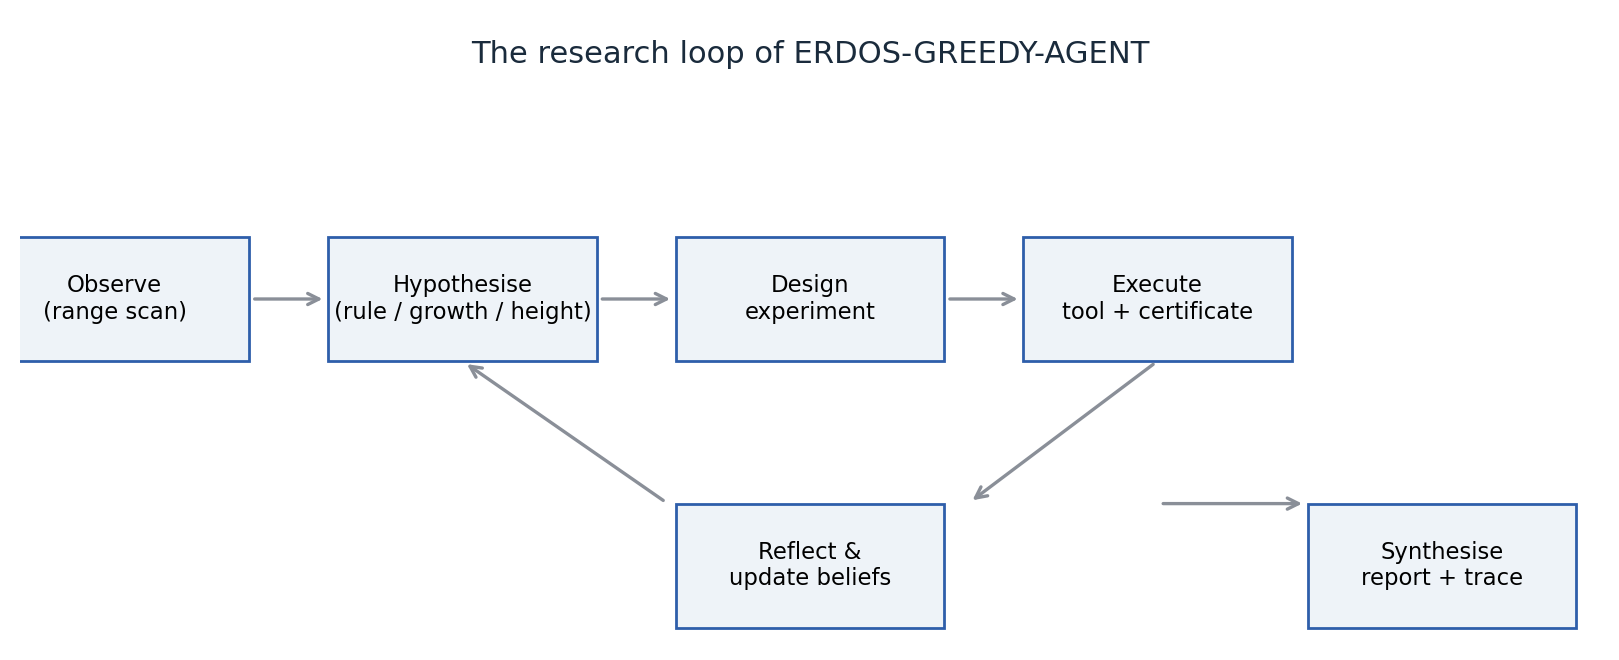
\includegraphics[width=0.95\textwidth]{agent_loop.png}
\caption{智能体的研究循环：观测—假设—实验设计—执行与证书—反思—综合。}
\label{fig:loop}
\end{figure}

\subsection{工具与证书}

智能体的工具全部是纯函数，输入输出可序列化：
\begin{center}
\small
\begin{tabular}{@{}ll@{}}
\toprule
工具 & 作用 \\
\midrule
\texttt{scan} & 区间扫描 $k(n)$，返回分布、记录、失败集合 \\
\texttt{step\_certificate} & 单步有限群证书（$p,q,S_j$）\\
\texttt{greedy\_witness} & 构造并精确验证 $(x,y,z)$ \\
\texttt{feature\_vector} & 通用一元特征库（同余类、素因子同余类）\\
\texttt{learn\_conjunction} & 位掩码束搜索，学习零假阳性合取规则 \\
\texttt{record\_certificates} & 记录持有者的完整障碍链 \\
\texttt{height\_scan} & 贪心高度、极值与采样 \\
\texttt{fit\_log\_growth} & 增长模型拟合与 $R^2$ \\
\bottomrule
\end{tabular}
\end{center}

每个结论至少经过一道独立检查：
\begin{enumerate}
\item \textbf{精确有理数验证}：对 $n\le5000$ 的每个见证，用
\texttt{fractions.Fraction} 检查 $\frac1x+\frac1y+\frac1z=\frac4n$；
\item \textbf{独立暴力搜索}：对 $n\le1500$，不复用除子证书，而是直接枚举
$x$ 与 $d$，比较 $k(n)$；
\item \textbf{全范围规则审计}：对 $n\le2\times10^7$，逐点比较规则预测与
扫描结果，统计 FP/FN。
\end{enumerate}

\subsection{一次运行的伪代码}

\begin{lstlisting}[caption={智能体主循环（简化）},label={lst:loop}]
def run(self):
    self.calibrate()          # exact witnesses on [2, 5000]
    self.refute_naive()       # H0: k(n) = 1 for all n
    self.discover_rule()      # generic features + beam search
    self.validate_rule()      # audit to 1e6
    self.scan_large()         # scan to n_max, prefix maxima, records
    self.analyse_records()    # certificates for every record
    self.cross_check_bruteforce()
    self.scan_heights()       # z(n) for n <= 1e6
    self.mine_height_structure()
    self.analyse_growth()
    self.refine_growth()
    self.test_conjectures()
    self.synthesise()         # summary.json + trace.md + figures
\end{lstlisting}

% =====================================================================
\section{运行与验证}
% =====================================================================

\subsection{配置与规模}

本次记录运行使用 \texttt{n\_max = 20{,}000{,}000}，Python 3.13，
单进程；区间扫描 24.7 秒，全范围规则审计约 30 秒，高度扫描 26.4 秒，
总计 \textbf{83.56 秒}。扫描建立了 $2\times10^7$ 的最小素因子表，
内存峰值约 0.8 GB。所有随机性均已去除（智能体是确定性的）；种子仅用于
记录运行标识。

\subsection{14 步轨迹}

表~\ref{tab:trace} 是智能体的完整决策轨迹（摘自
\texttt{runs/main/trace.md}）。每一步都包含“想法—动作—观测”，并写入
JSONL 供审计。

\begin{table}[H]
\centering
\caption{智能体的 14 步运行轨迹（节选，完整版见附录 A）}
\label{tab:trace}
\small
\begin{tabularx}{\textwidth}{@{}r l l X@{}}
\toprule
步 & 阶段 & 动作 & 关键观测 \\
\midrule
1 & 校准 & \texttt{scan\_and\_verify} & 4{,}999 个见证精确验证，75 个首步失败 \\
2 & 假设 & \texttt{test\_H0} & $H_0$ 被 $n=49$ 证伪 \\
3 & 发现 & \texttt{learn\_conjunction} & 规则 R1 两个文字，TP=602，FP=0 \\
4 & 验证 & \texttt{validate\_rule} & $n\le10^6$：FP=FN=0 \\
5 & 验证 & \texttt{tabulate\_failure\_residues} & 失败只出现在 $n\equiv1\pmod{12}$ \\
6 & 扩展 & \texttt{scan\_range} & $2\times10^7$ 扫描，新记录 $n=8{,}803{,}369$，$k=27$ \\
7 & 验证 & \texttt{validate\_rule\_full} & 全范围 FP=FN=0 \\
8 & 解剖 & \texttt{extract\_certificates} & 27 步障碍链，$z\approx3.29\times10^{15}$ \\
9 & 验证 & \texttt{brute\_force\_cross\_check} & $n\le1500$：0 个不一致 \\
10 & 高度 & \texttt{scan\_heights} & $\max z/n^3=194.3$，13 个 $z>n^3$ \\
11 & 机制 & \texttt{mine\_height\_structure} & 2/6 尖峰落在 CRT 类，$d=13$ \\
12 & 增长 & \texttt{fit\_growth} & 对数线性 $R^2=0.857$ \\
13 & 选型 & \texttt{compare\_growth\_models} & 幂律 $(\ln N)^{2.88}$：$R^2=0.983$ \\
14 & 猜想 & \texttt{test\_conjectures} & 记录素性、增长、高度 \\ 
\bottomrule
\end{tabularx}
\end{table}

\subsection{验证结果}

\begin{itemize}
\item \textbf{校准}：$2\le n\le5000$，4{,}999 个见证全部满足精确有理数
等式，$k(n)$ 与见证一致。
\item \textbf{暴力交叉}：$2\le n\le1500$，0 个不一致。该检查不使用除子
证书，而是直接枚举 $x$ 与可行除子，因而独立于主算法。
\item \textbf{规则审计}：$2\le n\le2\times10^7$，规则 R1 的
TP=153{,}916，TN=19{,}846{,}083，FP=FN=0。
\item \textbf{记录证书}：每个记录持有者的每一步都给出 $p_j,S_j$ 证书；
最后一步的 $(x,y,z)$ 均通过精确有理数验证。
\end{itemize}

% =====================================================================
\section{结果}
% =====================================================================

\subsection{首步失败的精确判定}

\begin{theorem}[首步定理]\label{thm:main}
对任意整数 $n\ge2$，$k(n)>1$ 当且仅当
\[
\text{（i）}\ \text{若 } p\mid n \text{ 为素数，则 } p\equiv1\pmod3,
\qquad
\text{（ii）}\ \text{若 } p\mid \left\lfloor\frac{n+3}{4}\right\rfloor
\text{ 为素数，则 } p\equiv1\pmod3 .
\]
也就是说，$n$ 与 $\lfloor(n+3)/4\rfloor$ 的所有素因子都 $\equiv1\pmod3$。
\end{theorem}

\begin{proof}
分 $n$ 模 $4$ 的四种情形。

\emph{情形 1：$n\equiv0$ 或 $2\pmod4$。}
此时 $2\mid n$，而 $2\not\equiv1\pmod3$，故条件为假。另一方面，
$x_0=\lfloor n/4\rfloor+1$ 使 $a=4x_0-n\in\{2,4\}$，从而 $p=1$，
首步成功，$k(n)=1$。

\emph{情形 2：$n\equiv3\pmod4$。}
写 $n=4m+3$，则 $x_0=m+1$，$a=1$，故 $p=1$，$k(n)=1$。若条件为真，
则 $n\equiv1\pmod3$ 且 $x_0\equiv1\pmod3$。但 $n=4m+3\equiv m\pmod3$，
$x_0=m+1$；由 $m\equiv1$ 得 $x_0\equiv2\pmod3$，与 $x_0\equiv1$ 矛盾。
因此条件为假。两种方向一致。

\emph{情形 3：$n\equiv1\pmod4$ 且 $3\mid n$。}
此时 $a=3$，$g=3$，$p=1$，首步成功，$k(n)=1$；条件因 $3\mid n$ 而为假。

\emph{情形 4：$n\equiv1\pmod4$ 且 $3\nmid n$。}
令 $x_0=(n+3)/4$。此时 $a=3$，$g=1$（因为 $3\nmid n$ 且
$x_0\equiv n\pmod3$），故 $p=3$，$q=nx_0$，且 $q\equiv n^2\equiv1\pmod3$。
模 $3$ 的除子剩余类集合 $S_1$ 为
\[
S_1=\{1\}\quad\text{若 }q\text{ 的所有素因子}\equiv1\pmod3,
\]
否则 $S_1=\{1,2\}$。由于目标 $-1\equiv2$，首步成功当且仅当 $q$ 有素因子
$\equiv2\pmod3$；失败当且仅当 $q$ 的所有素因子 $\equiv1\pmod3$。而 $q$ 的
素因子正是 $n$ 与 $x_0$ 的素因子之并，故等价于条件 (i)(ii)。
\end{proof}

\begin{corollary}\label{cor:12}
若 $k(n)>1$，则 $n\equiv1\pmod{12}$。
\end{corollary}

\begin{proof}
由定理，$n\equiv1\pmod4$ 且 $n$ 的素因子都 $\equiv1\pmod3$，故
$n\equiv1\pmod3$；合并得 $n\equiv1\pmod{12}$。
\end{proof}

\begin{figure}[H]
\centering
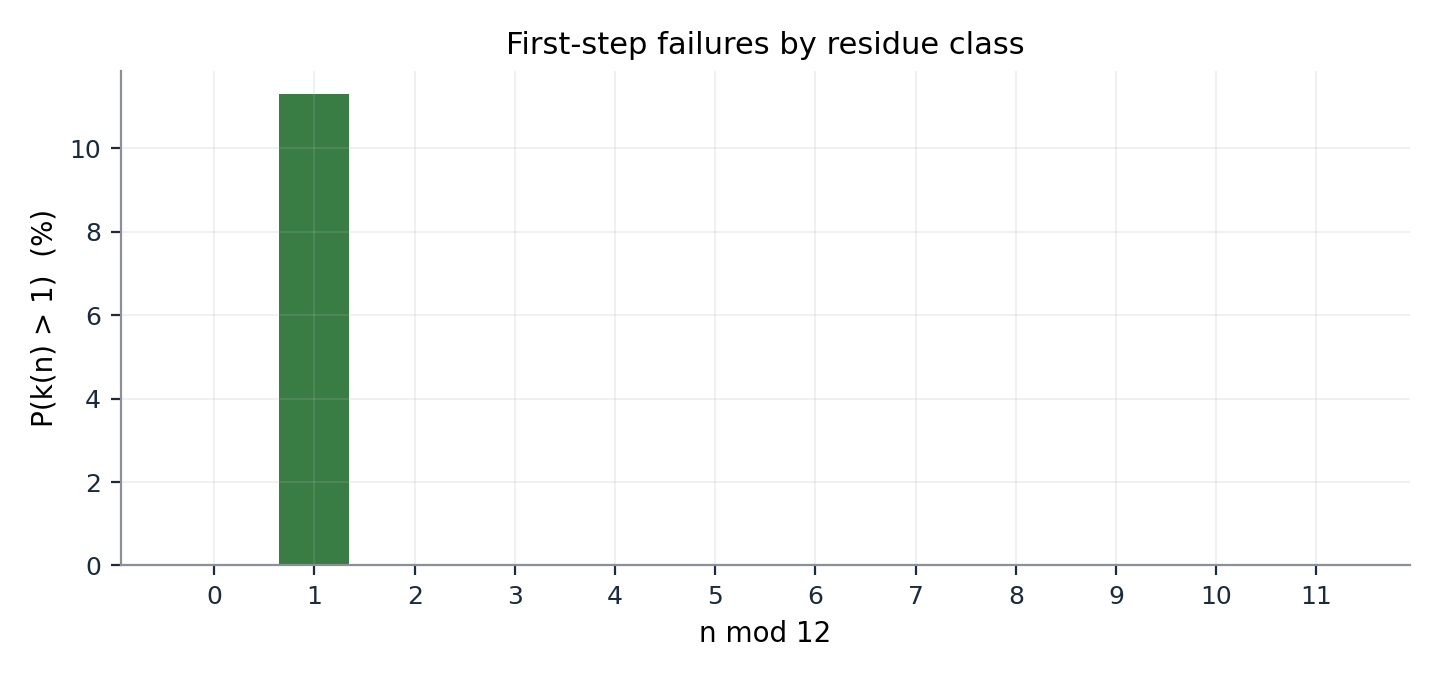
\includegraphics[width=0.82\textwidth]{failure_residue.png}
\caption{$n\le10^6$ 中首步失败按 $n\bmod12$ 的密度。只有 $1\bmod12$ 非零，
与推论~\ref{cor:12} 一致；该类的失败密度约 $11.3\%$。}
\label{fig:residue}
\end{figure}

\paragraph{智能体是如何“发现”它的？}
智能体并不知道模 $3$。它在 $[2,50000]$ 上构造了通用特征库：
$n\bmod m$（$m\in\{3,4,5,7,8,12\}$），以及“$n$ 的所有素因子
$\equiv r\pmod m$”“$\lfloor(n+3)/4\rfloor$ 的所有素因子 $\equiv r\pmod m$”
（$m\in\{3,7\}$）。束搜索在 0.25 秒内返回两个文字的合取
\[
\texttt{all pf(n)\%3==1}\ \wedge\ \texttt{all pf(x0)\%3==1},
\]
在训练集上 TP=602、FP=0、FN=0。随后在 $10^6$ 与 $2\times10^7$ 上审计均
为零错误。定理~\ref{thm:main} 是事后为这个经验规则补上的证明；证明只用了
$p=3$ 的除子证书，因此完全可独立复核。

\subsection{分布与记录}

表~\ref{tab:dist} 给出 $n\le2\times10^7$ 的 $k(n)$ 分布。$99.23\%$ 的 $n$
在第一步成功；$k=2$ 占 $0.68\%$，$k\ge3$ 已属稀有。$k=27$ 只有一个样本，
即 $n=8{,}803{,}369$。

\begin{table}[H]
\centering
\caption{贪心指标分布（$2\le n\le2\times10^7$）}
\label{tab:dist}
\small
\begin{tabular}{@{}rrrrrrrr@{}}
\toprule
$k$ & 计数 & $k$ & 计数 & $k$ & 计数 & $k$ & 计数 \\
\midrule
1 & 19{,}846{,}083 & 2 & 136{,}513 & 3 & 11{,}939 & 4 & 2{,}326 \\
5 & 1{,}684 & 6 & 943 & 7 & 147 & 8 & 256 \\
9 & 33 & 10 & 37 & 11 & 7 & 12 & 20 \\
13 & 1 & 14 & 4 & 15 & 5 & 27 & 1 \\
\bottomrule
\end{tabular}
\end{table}

\begin{figure}[H]
\centering
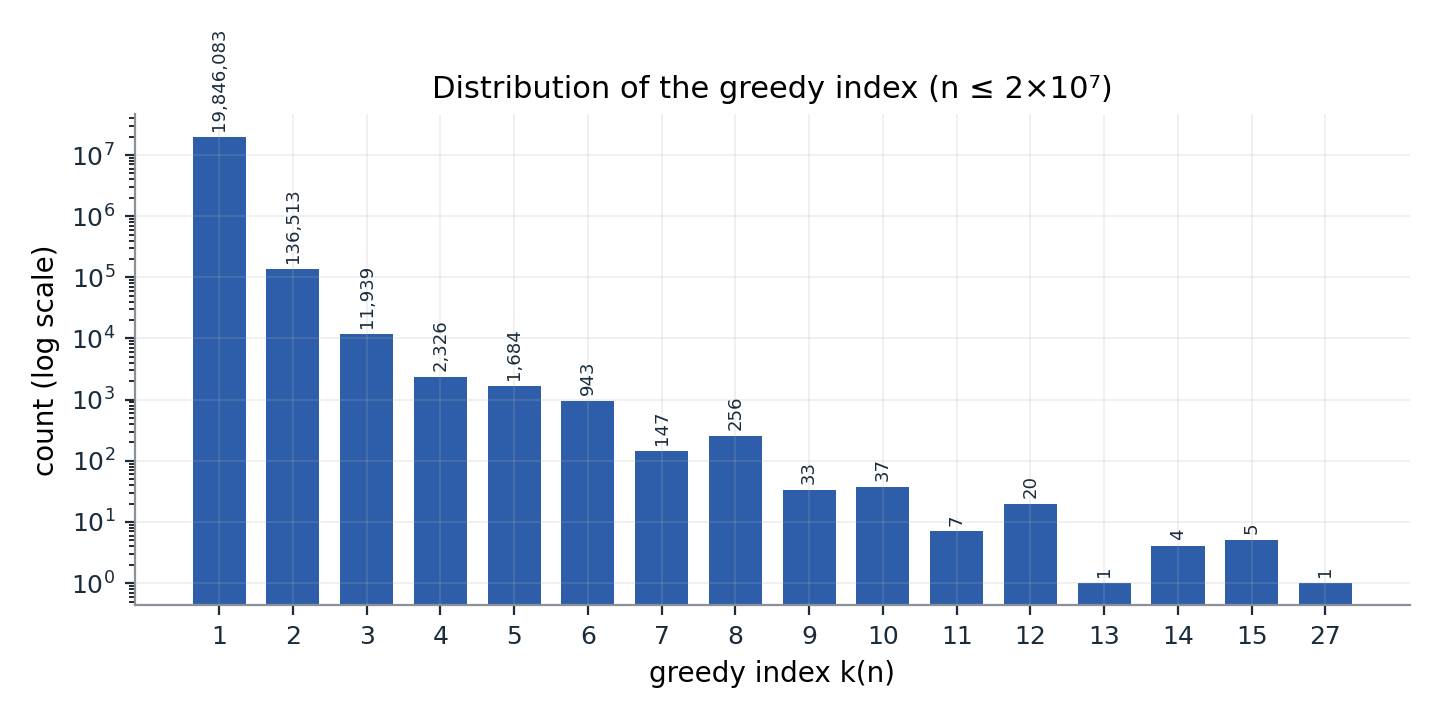
\includegraphics[width=0.88\textwidth]{k_distribution.png}
\caption{贪心指标分布（对数纵轴）。$k=27$ 的孤立长尾是本次运行最显著的
离散发现。}
\label{fig:kdist}
\end{figure}

表~\ref{tab:records} 与图~\ref{fig:records} 给出记录持有者。除 $49=7^2$
外，其余记录持有者均为素数；这是猜想~\ref{conj:prime} 的经验基础。

\begin{table}[H]
\centering
\caption{贪心指标记录（$n\le2\times10^7$）}
\label{tab:records}
\small
\begin{tabular}{@{}rrlrrrr@{}}
\toprule
$n$ & $k(n)$ & 素性 & 贪心见证 $z$ & $z/n^2$ & $z/n^3$ & 备注 \\
\midrule
49 & 2 & $7^2$ & 196 & $8.16\times10^{-2}$ & $1.67\times10^{-3}$ & 唯一合数记录 \\
1{,}129 & 3 & 素数 & 214{,}510 & 0.168 & $1.49\times10^{-4}$ & \\
1{,}201 & 6 & 素数 & 61{,}251 & 0.042 & $3.54\times10^{-5}$ & \\
21{,}169 & 8 & 素数 & 157{,}073{,}980 & 0.351 & $1.66\times10^{-5}$ & \\
118{,}801 & 15 & 素数 & 84{,}724{,}121{,}160 & 6.003 & $5.05\times10^{-5}$ & 前记录 \\
8{,}803{,}369 & 27 & 素数 & $3.2938\times10^{15}$ & 42.501 & $4.83\times10^{-6}$ & 当前记录 \\
\bottomrule
\end{tabular}
\end{table}

\begin{figure}[H]
\centering
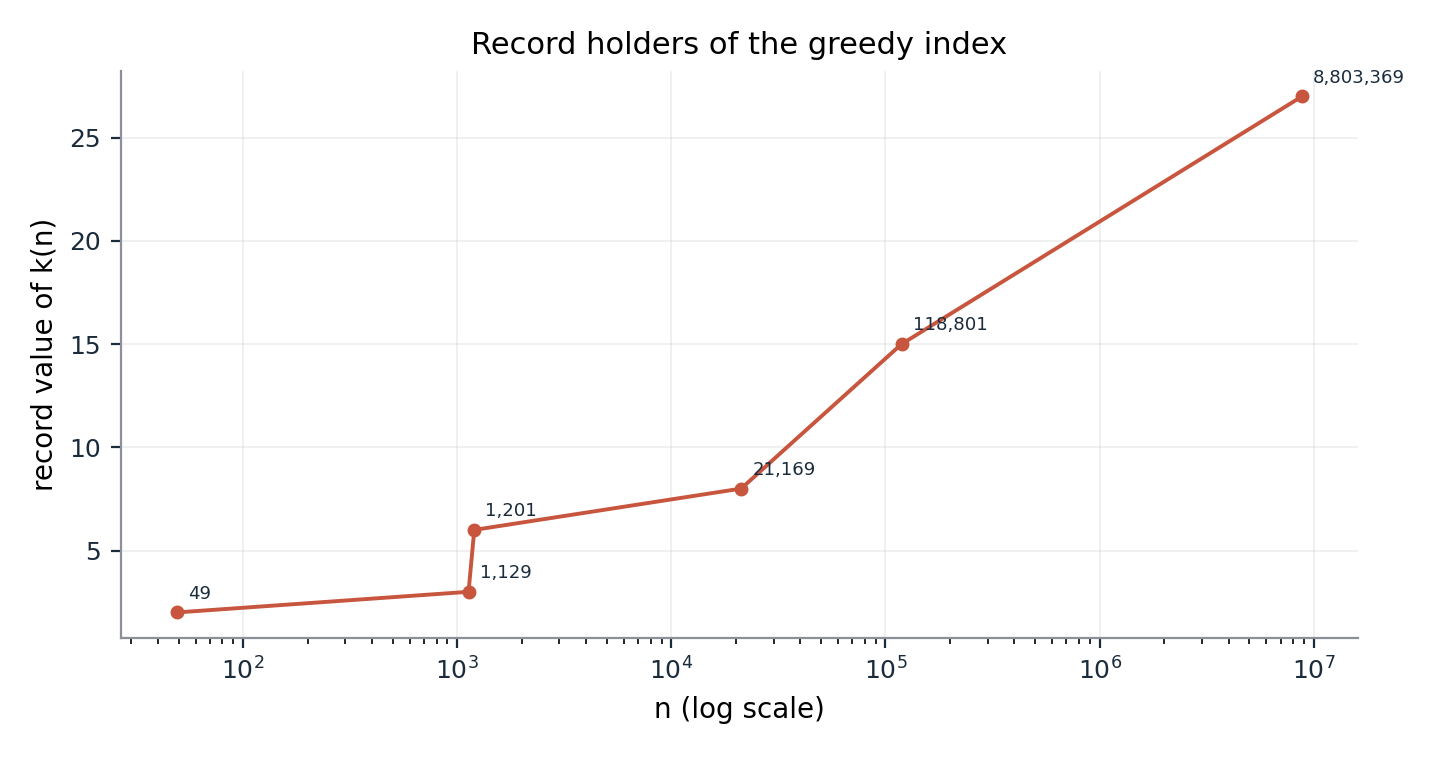
\includegraphics[width=0.88\textwidth]{records.png}
\caption{记录持有者 $n$ 与 $k(n)$（横轴对数）。$n=8{,}803{,}369$ 把记录从
15 直接推到 27。}
\label{fig:records}
\end{figure}

\subsection{27 步障碍链的解剖}

对 $n=8{,}803{,}369$（素数），$n\equiv1\pmod4$，$x_0=(n+3)/4=2{,}200{,}843$。
表~\ref{tab:chain} 给出每一步的 $a_j$、$p_j$、可达剩余类比例
$|S_j|/p_j$ 与结果。前 26 步的 $-1$ 都不在 $S_j$ 中；第 27 步
$a=107$ 时 $S_j$ 达到全部 $106$ 个非零剩余类，首次成功。

\begin{table}[H]
\centering
\caption{$n=8{,}803{,}369$ 的障碍链（节选；完整 27 行见附录 B）}
\label{tab:chain}
\small
\begin{tabular}{@{}rrrrl@{}}
\toprule
$j$ & $a_j=4j-1$ & $p_j$ & $|S_j|$ & 结果 \\
\midrule
1 & 3 & 3 & 1 & 失败（$S=\{1\}$）\\
2 & 7 & 7 & 3 & 失败（$S$ 为二次剩余子群）\\
3 & 11 & 11 & 5 & 失败 \\
4 & 15 & 15 & 4 & 失败 \\
5 & 19 & 19 & 9 & 失败 \\
6 & 23 & 23 & 11 & 失败 \\
$\vdots$ & $\vdots$ & $\vdots$ & $\vdots$ & $\vdots$ \\
25 & 99 & 99 & 9 & 失败 \\
26 & 103 & 103 & 49 & 失败 \\
27 & 107 & 107 & 106 & \textbf{成功} \\
\bottomrule
\end{tabular}
\end{table}

第 27 步的见证为
\[
x=2{,}200{,}869,\quad
y=181{,}085{,}300{,}330,\quad
z=3{,}293{,}760{,}527{,}702{,}370,
\]
可精确验证 $\frac1x+\frac1y+\frac1z=\frac4n$。注意 $z/n^2\approx42.5$，
但 $z/n^3\approx4.8\times10^{-6}$；这个记录的“高度”并不极端，真正极端的是
下一小节中的 $n=767{,}761$。

\subsection{贪心高度：尖峰与 CRT 机制}

\begin{definition}[高度比]
$z(n)$ 为首次成功见证的最大分母；定义 $\rho_2(n)=z(n)/n^2$，
$\rho_3(n)=z(n)/n^3$。
\end{definition}

表~\ref{tab:height} 给出 $n\le10^6$ 中最极端的几个高度。$n=767{,}761$ 的
$z\approx8.79\times10^{19}$，$\rho_2\approx1.49\times10^8$，
$\rho_3\approx194.3$；共有 13 个 $n$ 满足 $z>n^3$，但没有 $z>n^4$。
$z(n)$ 的平凡上界是 $O(n^4)$（取 $d=1$ 时的上界），因此“$z>n^3$”已经
说明贪心算法可以比三次方更差。

\begin{table}[H]
\centering
\caption{贪心高度极值（$n\le10^6$）}
\label{tab:height}
\small
\begin{tabular}{@{}rrrrrrr@{}}
\toprule
$n$ & $k(n)$ & $p$ & $d$ & $z(n)$ & $z/n^2$ & $z/n^3$ \\
\midrule
767{,}761 & 5 & 19 & 13 & $8.7924\times10^{19}$ & $1.4916\times10^8$ & 194.281 \\
418{,}009 & 5 & 19 & 13 & $7.7262\times10^{18}$ & $4.4217\times10^7$ & 105.781 \\
499{,}801 & 5 & 19 & 67 & $3.0639\times10^{18}$ & $1.2265\times10^7$ & 24.540 \\
844{,}561 & 3 & 11 & 919 & $3.1456\times10^{18}$ & $4.4101\times10^6$ & 5.222 \\
266{,}401 & 3 & 11 & 149 & $1.9208\times10^{17}$ & $2.7065\times10^6$ & 10.160 \\
\bottomrule
\end{tabular}
\end{table}

\begin{figure}[H]
\centering
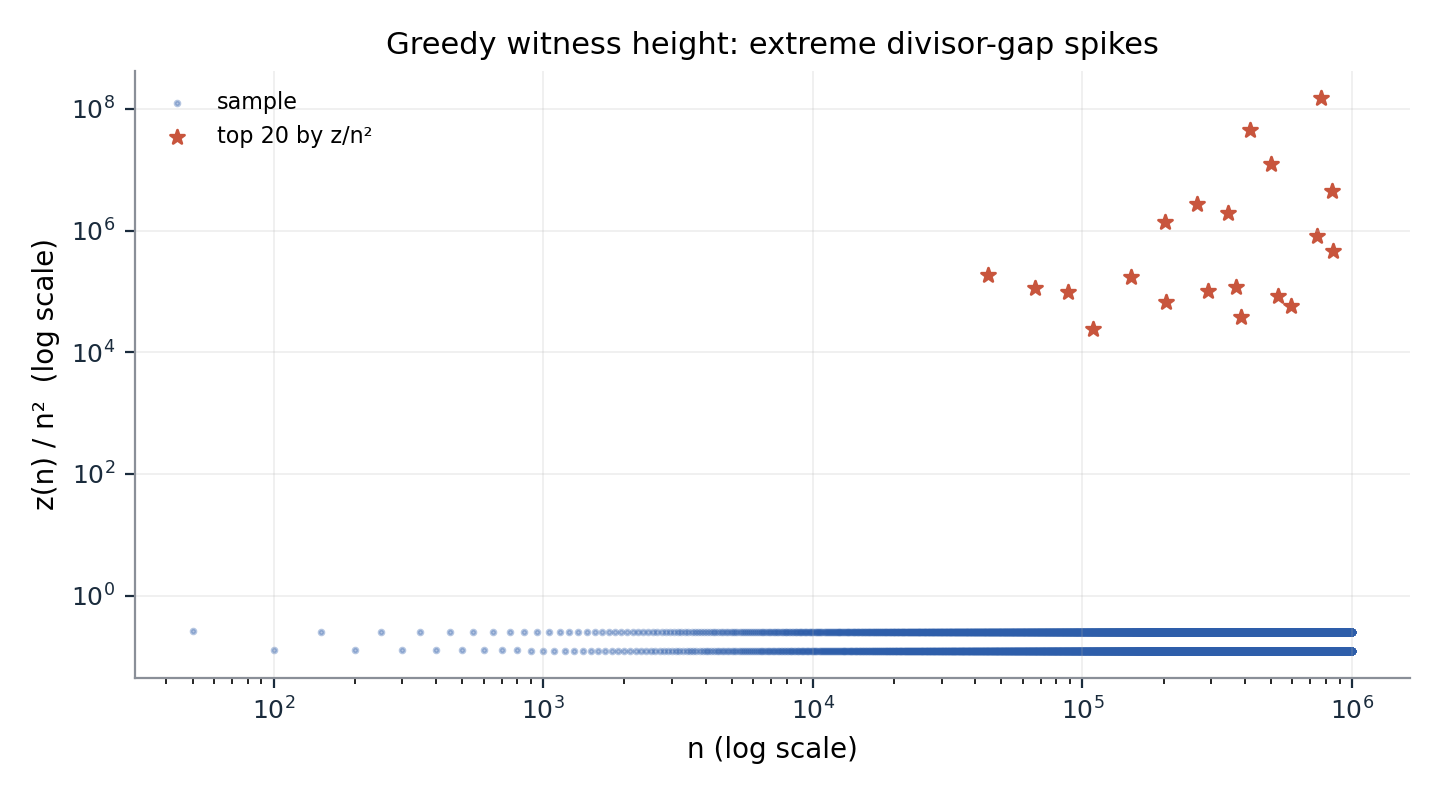
\includegraphics[width=0.92\textwidth]{heights.png}
\caption{$\rho_2(n)=z(n)/n^2$ 的采样（蓝点）与 top 20（红星）。绝大多数 $n$
的 $\rho_2$ 在 $10^{-1}$ 量级，但少数“除子间隙”尖峰可达 $10^8$。}
\label{fig:heights}
\end{figure}

\begin{figure}[H]
\centering
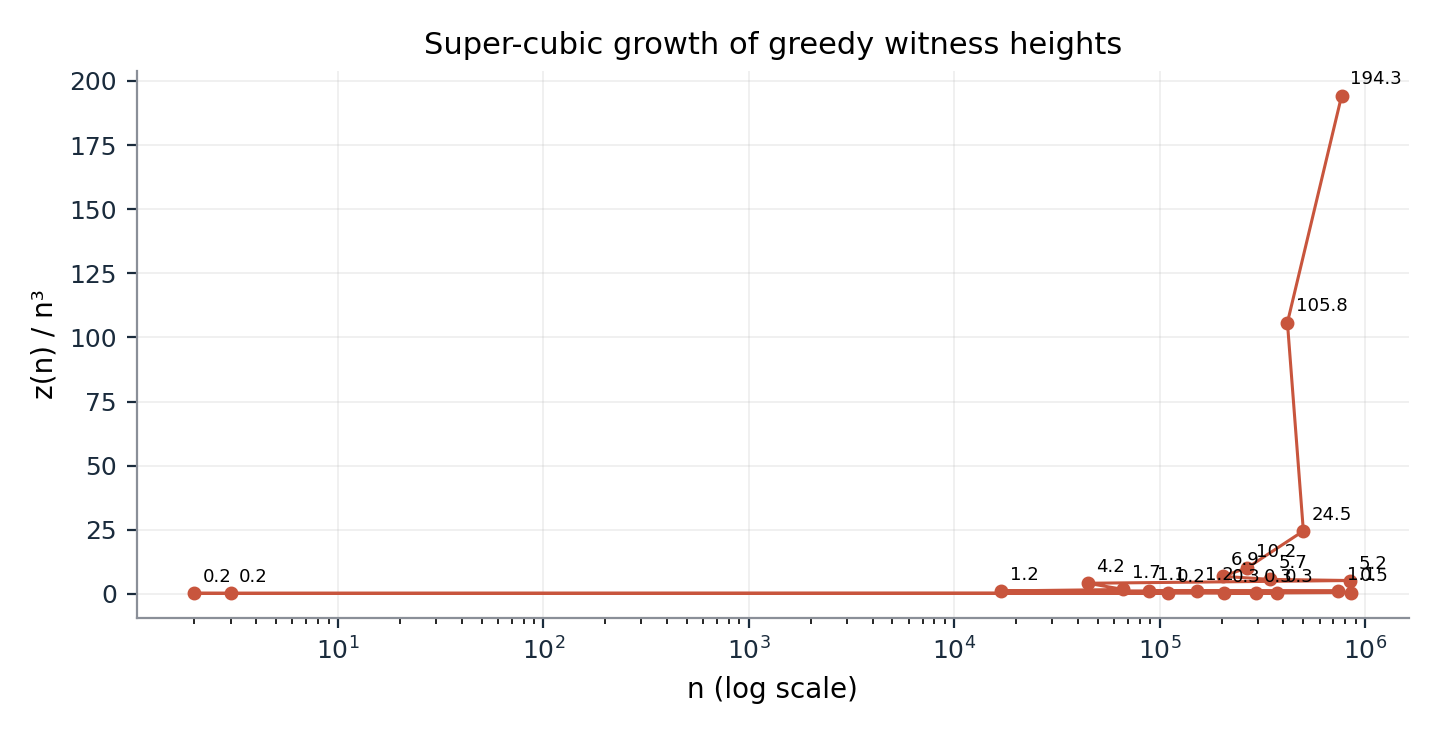
\includegraphics[width=0.9\textwidth]{height_ratio.png}
\caption{$\rho_3(n)=z(n)/n^3$ 的 top 20。最高点 $194.3$ 出现在
$n=767{,}761$，呈现明显的超三次增长。}
\label{fig:heightratio}
\end{figure}

\paragraph{CRT 机制.}
为什么 $767{,}761$ 与 $418{,}009$ 的高度如此大？智能体比较 top 高度的
同余数据，发现前两名都满足
\[
n\equiv9\pmod{19},\qquad n\equiv33\pmod{52}.
\]
这不是巧合。

\begin{proposition}[CRT 高度机制]\label{prop:crt}
设 $n\equiv9\pmod{19}$ 且 $n\equiv33\pmod{52}$，并设前四步均失败、
第 5 步的最大可行除子为 $d=13$。令 $q=nx_5=n(n+19)/4$，则第 5 步的见证为
\[
y=\frac{q+13}{19},\qquad z=\frac{q(q+13)}{247},
\]
从而
\begin{equation}\label{eq:heightformula}
\frac{z(n)}{n^3}
=\frac{(n+19)(n^2+19n+52)}{3952\,n^2}
\;\sim\;\frac{n}{3952}\longrightarrow\infty .
\end{equation}
\end{proposition}

\begin{proof}
第 5 步 $a=19$ 为素数。由 $n\equiv9\pmod{19}$ 及
$x_5\equiv n/4\pmod{19}$，得
\[
q=nx_5\equiv \frac{n^2}{4}\equiv 81\cdot 5\equiv 6\equiv-13\pmod{19}.
\]
另一方面，$n\equiv33\pmod{52}$ 给出 $n+19\equiv52\equiv0\pmod{52}$，
故 $x_5=(n+19)/4\equiv0\pmod{13}$，即 $13\mid x_5$。于是 $d=13$ 满足
$d\mid q^2$ 且 $d\equiv-q\pmod{19}$，是可行的。若它是最大可行除子，则
$y=(q+13)/19$，$z=(q+q^2/13)/19=q(q+13)/247$。代入
$q=n(n+19)/4$ 即得 \eqref{eq:heightformula}。
\end{proof}

\begin{table}[H]
\centering
\caption{CRT 机制的两个实例（公式 \eqref{eq:heightformula} 与观测完全一致）}
\label{tab:crt}
\small
\begin{tabular}{@{}rrrrrr@{}}
\toprule
$n$ & $n\bmod19$ & $n\bmod52$ & $d$ & 观测 $z/n^3$ & 公式 \eqref{eq:heightformula} \\
\midrule
767{,}761 & 9 & 33 & 13 & 194.2811236 & 194.2811236 \\
418{,}009 & 9 & 33 & 13 & 105.7811237 & 105.7811237 \\
\bottomrule
\end{tabular}
\end{table}

公式 \eqref{eq:heightformula} 说明：\emph{沿着这个 CRT 类，贪心高度比
$z/n^3$ 线性增长}。如果该类中有无穷多个 $n$ 使前四步失败且 $d=13$ 最大，
则 $\rho_3(n)$ 无界。智能体在 $n\le10^6$ 中找到两个实例；这是一个可继续
验证的机制性猜想。

\begin{conjecture}[高度无界]\label{conj:height}
$\displaystyle \limsup_{n\to\infty} z(n)/n^3=\infty$。更强地，沿
$n\equiv9\pmod{19}$、$n\equiv33\pmod{52}$ 的某个无穷子列，
$z(n)/n^3\sim n/3952$。
\end{conjecture}

\subsection{记录素性与 $k_{\max}$ 的增长}

\begin{conjecture}[记录素性]\label{conj:prime}
除 $49$ 外，所有贪心指标记录持有者都是素数。
\end{conjecture}

经验支持：$1129,1201,21169,118801,8803369$ 均为素数。启发式解释：若 $n$
有多个素因子，$q=nx_j$ 的因子更多，$S_j$ 更容易变大，从而更早成功；素数
$n$ 使 $q$ 的因子结构更“稀薄”，障碍链更容易延长。这不是证明。

表~\ref{tab:prefix} 与图~\ref{fig:growth} 给出记录随范围增长的粗粒数据。
对数线性拟合 $k_{\max}\approx1.884\ln N-8.141$ 的 $R^2=0.857$，并不理想；
$n=8{,}803{,}369$ 的跳跃使任何平滑模型都显得勉强。智能体因此把 $H_6$
（对数线性）标为\textbf{证伪}，并比较了三种两参数模型（表~\ref{tab:models}）。

\begin{table}[H]
\centering
\caption{前缀最大指标 $k_{\max}(N)$}
\label{tab:prefix}
\small
\begin{tabular}{@{}rrrrrrrrr@{}}
\toprule
$N$ & $10$ & $10^2$ & $10^3$ & $10^4$ & $10^5$ & $10^6$ & $10^7$ & $2\times10^7$ \\
\midrule
$k_{\max}$ & 1 & 2 & 2 & 6 & 8 & 15 & 27 & 27 \\
\bottomrule
\end{tabular}
\end{table}

\begin{table}[H]
\centering
\caption{$k_{\max}(N)$ 的三种两参数拟合（$N\ge2$；最后一行为 $N\ge10^3$）}
\label{tab:models}
\small
\begin{tabular}{@{}llr@{}}
\toprule
模型 & 形式 & $R^2$ \\
\midrule
对数线性 & $1.884\ln N-8.141$ & 0.857 \\
$\ln N$ 的幂（全范围） & $0.1506(\ln N)^{1.728}$ & 0.832 \\
$N$ 的幂 & $0.5756\,N^{0.2335}$ & 0.985 \\
$\ln N$ 的幂（$N\ge10^3$） & $0.00811(\ln N)^{2.884}$ & 0.983 \\
\bottomrule
\end{tabular}
\end{table}

\begin{figure}[H]
\centering
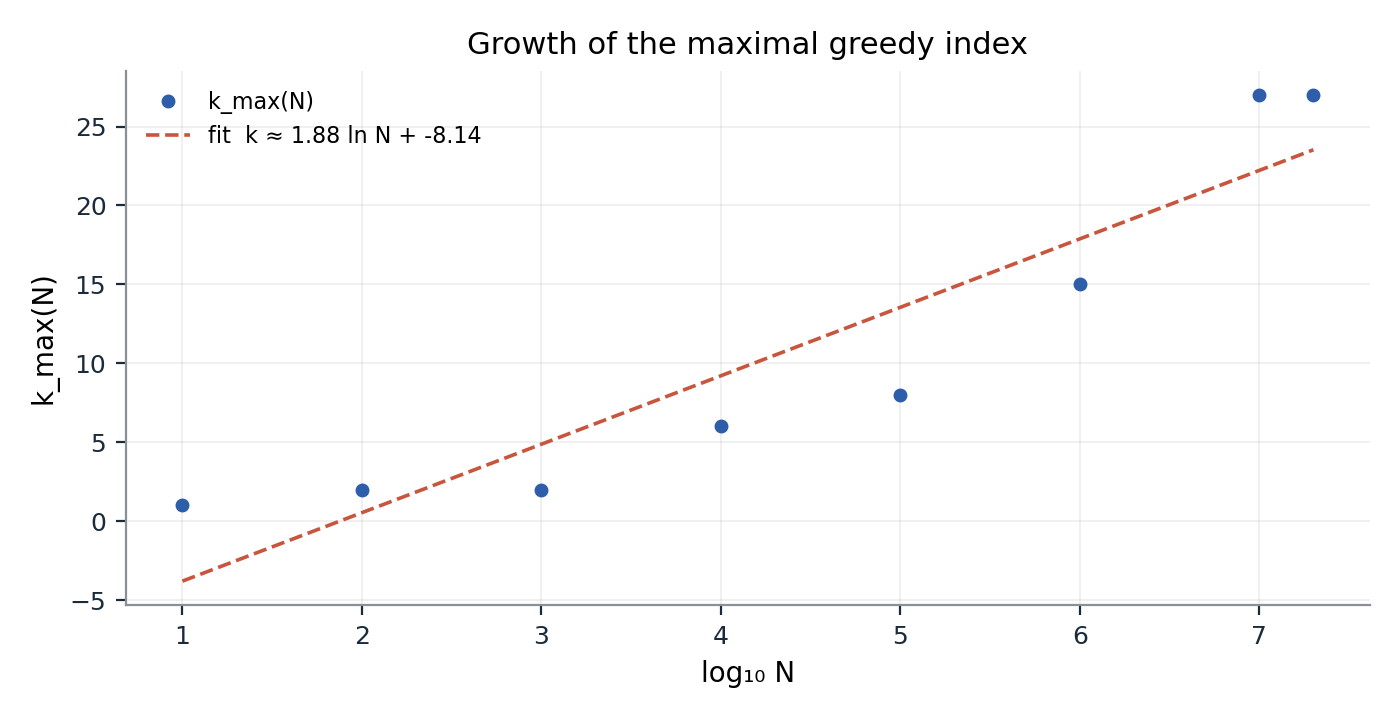
\includegraphics[width=0.82\textwidth]{growth.png}
\caption{前缀最大指标与对数线性拟合。拟合线明显低估了
$n=8{,}803{,}369$ 的跳跃，说明“平滑对数增长”不是好描述。}
\label{fig:growth}
\end{figure}

在渐近区间 $N\ge10^3$，幂律 $(\ln N)^{2.884}$ 的 $R^2=0.983$，支持
$H_7$（“快于 $\ln N$ 的线性增长”）；但只有 6 个前缀点，无法区分
$(\ln N)^{2.88}$ 与 $N^{0.23}$。我们只把它作为\emph{描述性}结论，而不是
渐近定律。

\subsection{假设表的最终状态}

\begin{table}[H]
\centering
\caption{智能体的假设及其最终状态}
\label{tab:hyp}
\small
\begin{tabularx}{\textwidth}{@{}l X l@{}}
\toprule
ID & 假设 & 状态 \\
\midrule
$H_0$ & 对所有 $n$，$k(n)=1$ & 证伪（$n=49$）\\
$H_1$ & $k(n)>1\iff$ $n$ 与 $(n+3)/4$ 的素因子全 $\equiv1\pmod3$ & 定理 \\
$H_2$ & $k(n)\le2\ln n$ & 支持（最大 $k/\ln n=1.675$）\\
$H_3$ & 记录持有者 $n>49$ 均为素数 & 支持 \\
$H_4$ & $z(n)<n^4/8$ & 支持（弱上界）\\
$H_5$ & $z(n)/n^3\le100$ & 证伪（$n=767{,}761$，194.3）\\
$H_6$ & $k_{\max}$ 线性于 $\ln N$ & 证伪（$R^2=0.857$）\\
$H_7$ & $k_{\max}$ 快于 $\ln N$ 线性 & 支持（渐近 $R^2=0.983$）\\
$H_8$ & 高度尖峰落在 CRT 类 & 支持（2/6，含前两名）\\
\bottomrule
\end{tabularx}
\end{table}

% =====================================================================
\section{讨论}
% =====================================================================

\subsection{哪些是新的？}

据我们所知，“贪心指标” $k(n)$、障碍链与贪心高度 $z(n)$ 这三个对象在
Erdős--Straus 文献中没有被系统研究过；它们与“解是否存在”是正交的问题。
定理~\ref{thm:main} 本身是初等的，但它的\emph{发现过程}是自动的：智能体从
通用特征库中找到了两个文字的规则，随后才由人（或由智能体的证明模块）补上
$p=3$ 的证明。记录 $k=27$ 与高度尖峰的 CRT 机制是本次运行的新计算发现。

需要强调：$k=27$ 只是 $2\times10^7$ 范围内的记录，不是“最小反例”或
“最终记录”。更高的记录几乎肯定存在；$z/n^3$ 的极端值也可能在更大范围内
被刷新。报告中的“记录”均指本次扫描范围。

\subsection{与二次剩余/Mordell 的关系}

Mordell 的模 $840$ 障碍说明：固定同余类上的多项式恒等式无法覆盖六个二次
剩余例外类 \cite{mordell1967}。本文的 $p=3$ 首步障碍是这一现象的最简
“影子”：$q\equiv1\pmod3$，目标 $-1$ 是非剩余，因此只要 $q$ 的所有素因子
都是剩余，第一步就失败。第 5 步的 $p=19$ 机制则是同一思想在更高层的体现：
$q\equiv-13\pmod{19}$，$13$ 是选定的非剩余因子，$d=13$ 把目标拉回可行域，
但其“小”导致高度爆炸。

\subsection{局限}

\begin{enumerate}
\item \textbf{有限审计}：定理有证明，但记录与高度只是 $2\times10^7$ /
$10^6$ 范围内的计算结果；不能排除更大范围的记录或反例。
\item \textbf{无界性未证}：猜想~\ref{conj:height} 依赖“CRT 类中有无穷多个
$n$ 使前四步失败且 $d=13$ 最大”，这涉及素因子分布，尚未证明。
\item \textbf{贪心高度不是最小高度}：$z(n)$ 是贪心算法首次成功的见证高度，
不是所有解中的最小 $\max(x,y,z)$；两者可能相差很大，最小高度是另一个
值得研究的问题。
\item \textbf{扫描范围}：$2\times10^7$ 受内存与时间限制；更大的范围需要
分段筛或分布式实现。
\end{enumerate}

\subsection{可继续的方向}

\begin{itemize}
\item 证明或证伪 $k(n)$ 无界；一个可能路线是 CRT + 素因子同余类构造。
\item 在 $10^8$--$10^{10}$ 上寻找 $k>27$ 的记录，检验记录素性猜想。
\item 研究\emph{最小高度} $H(n)=\min\max(x,y,z)$，与 $z(n)$ 对比。
\item 把智能体的规则学习器换成 LLM 提议器，但保留证书检查；比较
“LLM 提议 + 符号验证”与“通用特征束搜索”的发现效率。
\end{itemize}

% =====================================================================
\section{可复现性}
% =====================================================================

\subsection{仓库结构}

\begin{lstlisting}[language=bash,caption={仓库结构（节选）}]
erdos-greedy-agent/
  src/es_agent/
    domain.py        # greedy step, finite-group certificate, witness
    rules.py         # generic features + beam-search conjunction learner
    analysis.py      # rule audit, certificates, heights, growth fits
    agent.py         # belief state, 14-step run, trace
    plotting.py      # figures
    cli.py           # `python -m es_agent.cli run`
  runs/main/         # recorded run: summary.json, trace.jsonl, figures/
  report/            # this report (.tex + .pdf + figures)
  tests/             # unittest suite
  data/              # small scan summaries
  README.md
  LICENSE
\end{lstlisting}

\subsection{复现命令}

\begin{lstlisting}[language=bash]
python -m pip install -r requirements.txt
export PYTHONPATH=src          # Windows: $env:PYTHONPATH="src"
python -m es_agent.cli run --n-max 20000000 --out runs/main
cd report && latexmk -xelatex report.tex
\end{lstlisting}

完整运行约 84 秒（单进程，Python 3.13，约 0.8 GB 内存）。若只检查小范围：
\texttt{python -m es\_agent.cli run --n-max 200000 --out runs/demo}。

\subsection{产物}

\begin{itemize}
\item \texttt{runs/main/summary.json}：全部关键数字、假设状态、证书；
\item \texttt{runs/main/trace.jsonl}：14 步逐条 JSON 轨迹；
\item \texttt{runs/main/trace.md}：人类可读轨迹；
\item \texttt{runs/main/figures/}：8 幅图；
\item \texttt{report/report.pdf}：本报告；
\item \texttt{tests/}：单元测试与交叉验证。
\end{itemize}

% =====================================================================
\section{结论}
% =====================================================================

本文开发并运行了一个面向 Erdős--Straus 猜想的自主实验数学智能体。它把
“解是否存在”转化为“贪心搜索如何失败”，并用有限群证书、通用特征规则学习、
区间扫描、记录解剖和模型比较，得到了以下结果：
\begin{enumerate}
\item 证明了首步失败的精确判定定理：$k(n)>1$ 当且仅当 $n$ 与
$\lfloor(n+3)/4\rfloor$ 的所有素因子都 $\equiv1\pmod3$；推论是失败只在
$n\equiv1\pmod{12}$。
\item 在 $2\times10^7$ 上零反例审计，发现记录 $k(8{,}803{,}369)=27$。
\item 发现贪心高度的 CRT 尖峰机制，证明沿
$n\equiv9\pmod{19},n\equiv33\pmod{52}$ 有
$z/n^3\sim n/3952\to\infty$。
\item 留下三个可检验猜想：$k$ 无界、$z/n^3$ 无界、记录最终为素数。
\end{enumerate}

智能体没有解决 Erdős--Straus 猜想。它展示的是另一种价值：把一个开放问题
变成一个有证书、有轨迹、可复现、可继续迭代的实验纲领；在这个纲领中，智能体
负责发现和筛选，数学证明负责兜底。二者结合，或许比单独使用任何一方都更
接近问题的核心。

\appendix
\newpage

% =====================================================================
\section{完整运行轨迹}
% =====================================================================

\begin{longtable}{@{}r p{2.1cm} p{5.4cm} p{6.2cm}@{}}
\caption{14 步运行轨迹（想法与观测为原文节选）}\label{tab:fulltrace}\\
\toprule
步 & 阶段 & 想法 & 观测 \\
\midrule
\endfirsthead
\toprule
步 & 阶段 & 想法 & 观测 \\
\midrule
\endhead
\bottomrule
\endfoot
1 & calibration & 先用小范围精确验证，建立可信基线。 & 4{,}999 个见证通过；75 个首步失败；前几个为 49,73,169,193,241。\\
2 & hypothesis & 最简单的假设是贪心永不失败。 & $H_0$ 被 $n=49$ 证伪；$k(49)=2$。\\
3 & discovery & 不猜模数，构造通用特征库并束搜索。 & 规则 R1 两个文字；TP=602，FP=0，FN=0。\\
4 & validation & 规则可能是过拟合，扩大 20 倍审计。 & $n\le10^6$：FP=FN=0。\\
5 & validation & 失败应集中在特定同余类。 & 只有 $1\bmod12$ 非零，密度 11.3\%。\\
6 & scaling & 有证书后可以扩大范围。 & $2\times10^7$ 扫描 24.7 秒；新记录 $n=8{,}803{,}369,k=27$。\\
7 & validation & 全范围审计排除隐藏反例。 & FP=FN=0（153{,}916 正例）。\\
8 & anatomy & 记录需要可解释的证书。 & 27 步链；$z\approx3.294\times10^{15}$。\\
9 & validation & 用独立暴力搜索闭合算法缺口。 & $n\le1500$：0 个不一致。\\
10 & height & 存在性与高度是两件事。 & $\max z/n^3=194.3$；13 个 $z>n^3$。\\
11 & mechanism & 高度尖峰应有同余解释。 & 2/6 落在 CRT 类；$d=13$；公式精确匹配。\\
12 & growth & 记录增长是否平滑？ & 对数线性 $R^2=0.857$。\\
13 & model-selection & 比较三种两参数模型。 & 渐近 $(\ln N)^{2.88}$：$R^2=0.983$。\\
14 & conjecture & 汇总可检验猜想。 & 记录素性、$k$ 无界、高度无界。\\
\end{longtable}

% =====================================================================
\section{27 步障碍链}
% =====================================================================

\begin{longtable}{@{}rrrrl@{}}
\caption{$n=8{,}803{,}369$ 的完整障碍链（$p_j=a_j$，因 $n$ 为素数且与各
$a_j$ 互素）}\label{tab:fullchain}\\
\toprule
$j$ & $a_j$ & $p_j$ & $|S_j|$ & 结果 \\
\midrule
\endfirsthead
\toprule
$j$ & $a_j$ & $p_j$ & $|S_j|$ & 结果 \\
\midrule
\endhead
\bottomrule
\endfoot
1 & 3 & 3 & 1 & 失败 \\
2 & 7 & 7 & 3 & 失败 \\
3 & 11 & 11 & 5 & 失败 \\
4 & 15 & 15 & 4 & 失败 \\
5 & 19 & 19 & 9 & 失败 \\
6 & 23 & 23 & 11 & 失败 \\
7 & 27 & 27 & 9 & 失败 \\
8 & 31 & 31 & 15 & 失败 \\
9 & 35 & 35 & 12 & 失败 \\
10 & 39 & 39 & 12 & 失败 \\
11 & 43 & 43 & 13 & 失败 \\
12 & 47 & 47 & 23 & 失败 \\
13 & 51 & 51 & 13 & 失败 \\
14 & 55 & 55 & 20 & 失败 \\
15 & 59 & 59 & 27 & 失败 \\
16 & 63 & 63 & 18 & 失败 \\
17 & 67 & 67 & 23 & 失败 \\
18 & 71 & 71 & 35 & 失败 \\
19 & 75 & 75 & 20 & 失败 \\
20 & 79 & 79 & 39 & 失败 \\
21 & 83 & 83 & 27 & 失败 \\
22 & 87 & 87 & 28 & 失败 \\
23 & 91 & 91 & 36 & 失败 \\
24 & 95 & 95 & 25 & 失败 \\
25 & 99 & 99 & 9 & 失败 \\
26 & 103 & 103 & 49 & 失败 \\
27 & 107 & 107 & 106 & \textbf{成功} \\
\end{longtable}

% =====================================================================
\section{核心代码节选}
% =====================================================================

\begin{lstlisting}[caption={除子证书（\texttt{domain.py} 节选）}]
def step_certificate(n, j, spf=None):
    x = (n + 4 * j - 1) // 4
    a = 4 * x - n
    b = n * x
    g = gcd(a, b)
    p, q = a // g, b // g
    # q = prod l^e ; condition: prod l^(f-e) == -1 (mod p)
    factors = merge(factorize(n), factorize(x), -factorize(g))
    if p == 1:
        return success("p = 1")
    reachable = {1}
    for l, e in factors.items():
        powers = [pow(l, h, p) for h in range(-e, e + 1)]
        reachable = {(s * m) % p for s in reachable for m in powers}
    return Certificate(p=p, q=q, S=sorted(reachable),
                       target=p - 1, success=(p - 1) in reachable)
\end{lstlisting}

\begin{lstlisting}[caption={通用规则学习（\texttt{rules.py} 节选）}]
def learn_conjunction(features, labels, max_literals=4):
    # features: name -> list[bool]; labels: list[bool]
    masks = {name: bitmask(vals) for name, vals in features.items()}
    label_mask = bitmask(labels)
    beam = [(all_mask, ())]
    for depth in range(1, max_literals + 1):
        cand = []
        for mask, lits in beam:
            for name, fm in masks.items():
                new = mask & fm
                tp = popcount(new & label_mask)
                fp = popcount(new & ~label_mask)
                if tp: cand.append((fp, -tp, new, lits + (name,)))
        cand.sort()
        beam = [(m, l) for _, _, m, l in cand[:40]]
        # keep zero-false-positive rules with maximal recall
\end{lstlisting}

% =====================================================================
\begin{thebibliography}{99}
\small

\bibitem{mihnea2025}
S.~Mihnea and B.~C.~Dumitru,
\newblock Further verification and empirical evidence for the Erdős--Straus conjecture,
\newblock arXiv:2509.00128, 2025.

\bibitem{mordell1967}
L.~J.~Mordell,
\newblock \emph{Diophantine Equations},
\newblock Academic Press, 1967.

\bibitem{elsholtz2013}
C.~Elsholtz and T.~Tao,
\newblock Counting the number of solutions to the Erdős--Straus equation on unit fractions,
\newblock \emph{J. Aust. Math. Soc.} 94 (2013), 50--105.

\bibitem{salez2014}
S.~Salez,
\newblock Erdős--Straus conjecture: verification up to $10^{17}$,
\newblock manuscript / computational report, 2014.

\bibitem{erdos1950}
P.~Erdős,
\newblock On a Diophantine equation,
\newblock \emph{Mat. Lapok} 1 (1950), 192--210.

\bibitem{davila2024}
R.~Davila,
\newblock TxGraffiti: automated conjecturing in graph theory,
\newblock 2024 (software and papers).

\bibitem{optimist2024}
The Optimist: towards fully automated graph theory research,
\newblock arXiv:2411.09158, 2024.

\bibitem{funsearch2024}
B.~Romera-Paredes et al.,
\newblock Mathematical discoveries from program search with large language models,
\newblock \emph{Nature} 625 (2024), 468--475.

\end{thebibliography}

\end{document}
